\documentclass[
	12pt,				% Tamanho da fonte
	openright,			% Capítulos começam em pág ímpar
	oneside,			% Para impressão em apenas um lado. Use 'twoside' para frente e verso
	a4paper,			% Tamanho do papel
	portuguese,			% Idioma adicional para hifenização
	brazil				% O idioma principal do documento
	]{abntex2}

% chktex 13  % Ignorar aviso sobre espaçamento entre sentenças

% --- PACOTES BÁSICOS ---
\usepackage[utf8]{inputenc}		% Codificação do documento
\usepackage[T1]{fontenc}		% Seleção de códigos de fonte
\usepackage{indentfirst}		% Indentação o primeiro parágrafo de cada seção
\usepackage{color}				% Controle de cores
\usepackage{graphicx}			% Inclusão de gráficos
\usepackage{microtype} 			% Para melhorias na justificação
\usepackage{amsmath}  % Essencial para fórmulas matemáticas
\usepackage{amsfonts} % Para símbolos como o de conjuntos (R, N, Z)
\usepackage{amssymb}  % Símbolos extras a
\usepackage{float}
\usepackage{placeins}
\graphicspath{{images/}}

% --- CONFIGURAÇÕES DE PACOTES ---
\usepackage{abntex2cite}   	% Citações padrão ABNT (Autor-data)

\hypersetup{
    colorlinks=false,
    hidelinks,      % Remove bordas, cores e sublinhados
    pdfborder={0 0 0}
}

% --- INFORMAÇÕES DO TCC ---
\titulo{Análise da Transição para Algorítmos criptográficos Pós-Quânticos nos modelos NIST}
\autor{Jean Victor Borges de Abreu}
\local{Petrópolis -Rio de Janeiro}
\data{2026}
\orientador{Nome do Orientador}
\instituicao{FACULDADE DE EDUCAÇÃO TECNOLÓGICA DO ESTADO DO RIO DE JANEIRO FAETERJ/PETRÓPOLIS}
\preambulo{Trabalho de Conclusão de Curso apresentado à}

% --- INÍCIO DO DOCUMENTO ---
\begin{document}

\imprimircapa

\imprimirfolhaderosto

\chapter{Resumo}

\chapter{Abstract}

\chapter{Lista de Figuras}
    \listoffigures
    
\chapter{Lista de Abreviaturas}

\boldmath{ABNT:\@ Associação Brasileira de Normas Técnicas}
\boldmath{CSPRNG:\@ Cryptographically Secure Pseudo Random Number Generator}
\boldmath{DRBG:\@ Deterministic Random Bit Generator}
\boldmath{FAETERJ:\@ Faculdade de Educação Tecnológica do Estado do Rio de Janeiro}
\boldmath{JEP:\@ JDK Enhancement Proposals}
\boldmath{KEM:\@ Key Encapsulation Mechanism}
\boldmath{LCG:\@ Linear Congruential Generator}
\boldmath{LWE:\@ Learning With Errors}
\boldmath{ML-KEM:\@ Module-Lattice-Based Key Encapsulation Mechanism}
\boldmath{NIST:\@ National Institute of Standards and Technology}
\boldmath{NRBG:\@ Non-deterministic Random Bit Generator}
\boldmath{PQC:\@ Post-Quantum Cryptography}
\boldmath{PRNG:\@ Pseudo Random Number Generator}
\boldmath{QRNG:\@ Quantum Random Number Generator}
\boldmath{TRNG:\@ True Random Number Generator}

% --- SUMÁRIO ---
\pdfbookmark[0]{\contentsname}{toc}
\tableofcontents
\cleardoublepage
% --- ELEMENTOS TEXTUAIS ---
\textual

\chapter{Introdução}

A onipresença da criptografia na infraestrutura digital moderna (internet, sistemas bancários, IoT e comunicações seguras).

\section{Contextualização do Tema}

Textos 

\section{Justificativa/Problema de Pesquisa}

O conflito entre o determinismo computacional e a necessidade de aleatoriedade em~sistemas criptográficos.

\section{Motivação/Hipotese e Ameaca Tecnológica}

O impacto da computação quântica --- especialmente por meio do Algoritmo de Shor --- sobre os modelos atuais de segurança e pseudoaleatoriedade.

\section{Objetivos}

Objetivo Geral: Analisar a evolução dos geradores pseudoaleatórios criptograficamente seguros frente à transição para a criptografia pós-quântica.
Objetivos Específicos:
Estudar PRNGs e CSPRNGs clássicos
Analisar o impacto dos algoritmos quânticos
Investigar os novos paradigmas de pseudoaleatoriedade baseados em reticulados
Avaliar a adoção desses conceitos no ecossistema Java


\section{Metodologia}

Pesquisa bibliográfica, análise documental de padrões criptográficos e estudo prático no ecossistema Java.

\chapter{FUNDAMENTOS DA ALEATORIEDADE EM COMPUTAÇÃO} % Capitulo 2


    \section{Entropia e Fontes de Incerteza}

        Captação de eventos físicos imprevisíveis como base para sistemas criptográficos seguros.

        Entropia é uma medida da aleatoriedade ou imprevisibilidade dos dados. 
        No contexto da criptografia, a entropia é usada para gerar 
        números aleatórios ou chaves que são essenciais para a comunicação segura e a criptografia. 
        Sem uma boa fonte de entropia, os protocolos criptográficos podem se tornar vulneráveis a ataques 
        que exploram a previsibilidade das chaves geradas.

        Na maioria dos sistemas operacionais, 
        a entropia é gerada pela coleta de eventos aleatórios de diversas fontes, 
        como interrupções de hardware, movimentos do mouse, 
        pressionamentos de teclas e atividade do disco. 
        Esses eventos são inseridos em um conjunto de entropia, 
        que é então usado para gerar números aleatórios quando necessário.

        Protocolos criptográficos, como SSL/TLS, SSH e IPsec, 
        dependem fortemente da entropia para gerar números aleatórios e chaves para criptografia, 
        autenticação e proteção de integridade.
        A aleatoriedade desses números é crucial para a segurança da comunicação. 
        Se um atacante conseguir prever os números aleatórios usados em um protocolo criptográfico, 
        ele poderá comprometer a confidencialidade, a integridade ou a autenticidade da comunicação.
        Se a chave mestra prévia for previsível ou tendenciosa, 
        um atacante poderá interceptar a mensagem criptografada, 
        descriptografá-la e obter acesso às chaves de sessão. 
        Isso permitiria ao atacante espionar a comunicação, 
        modificar os dados ou se passar pelo servidor.\nocite{6.2Entropia}

        Um tipo de entropia. É a entropia de ``Shannon''. Que utiliza umm tratamento probabilístico
        de uma função logarítmica.\cite{6.2shannonEntropia} Sendo sua formula:

        \begin{equation}
            H(X) = - \sum_{i=1}^{n} P(x_i) \log_b P(x_i)
            \label{eq:shannon_entropy}
        \end{equation}

        Em que:
        \begin{itemize}
            \item $H(X)$ é a entropia em bits;
            \item $p_i$ é a probabilidade de ocorrência do resultado $i$;
            \item $n$ é o número total de resultados possíveis.
        \end{itemize}

        Uma limitação determinística é em cima de um processador de maquina de estados finitos.
        Se acaso for utilizado as mesmas variáveis, o resultado permanece inalterado.\@ Onde se um invasor 
        tiver a certeza da seed de origem da criptografia. Ela por si mesma, não é aleatória. Para evitar tais acontecimentos
        se faz necessário que o software faça a captação da incerteza do mundo físico.

        A entropia deve ter força superior ou igual a segurança do sistema criptográfico. 
        Entropia adicional poder ser necessária para compensar a perda de entropia durante o processo de geração de chaves, mas não necessariamente adiona mais segurança.
        Ter mais entropia do que a quantidade avaliada é aceitavel, ter menos do que o recomendado pode ser fatal para a segurança do sistema criptográfico. 
        O comprimento minimo depende do mecanismo criptográfico específico e do nível de segurança desejado.
        A entrada de entropia e a seed resultante devem ser consistentes com a segurança dos dados protegidos pelo consumidor. 
        Em um modelo DRBG a seed e as chaves geradas deevem possuir o mesmo nivel de segurança, pois no modelo DRBG depende da entropia usada, seguindo o critério de segurança critico (CSP).%\nocite{NIST 800-90A, pg 18/19 8.6.3}



    \section{A Semente (Seed) como Elemento Crítico}

        Falar sobre esse ponto, pois vai ser utilizado na explicação dos protocolos tanto do funcionamento de verificação do NIST 800--22, do NIST IR 8547 e do NIST IR 7977 pos quantico 

        Uma sequência de bits usada como entrada para um gerador de números pseudoaleatórios (DRBG). A semente é a chave inicial, usada internamente para a concepção do DRBG. Sua entropia deve ser suficiente para garantir a segurança do DRBG.
        A semente é um elemento crítico, pois determina a sequência de números pseudoaleatórios gerados pelo DRBG.\@
        Se a semente for previsível ou tiver baixa entropia, o DRBG pode ser vulnerável a ataques que exploram essa fraqueza. Portanto, é essencial que a semente seja gerada a partir de uma fonte de entropia confiável.


        Uma sequência de bits usada como entrada para um mecanismo DRBG.\@ A semente determinará uma parte do interior estado do DRBG, e sua entropia deve ser suficiente para apoiar a força de segurança do DRBG
        Para obter uma seed suficientemente aleatória. Deve se submeter a uma estimativa de entropia para as saidas da fonte de ruido, baseada na propria fonte da entropia. Essa estimativa é denominada de $\mathit{H_{\text{submitter}}}$.
        Depois de possuir uma trilha de estimativas, a estimativa de entropia minima por amostra chamada de $\mathit{H_{\text{original}}}$ é determinada. 
        Se o tamanho for superior a 256 bits, ele precisara ser reduzido para menor ou igual a 256 bits.

        Se o conjunto de dados não for binário, é necessario uma entropia adicional em bit, denominada de $\mathit{H_{\text{bitstring}}}$ é estimada. O conjunto de dados sequencias possui L amostras, cada uma contendo N bits e é considerado uma cadeia de bits
        de tamanho $L \times N$. Após os primeiros 1.000.000 bits podem vir a serem desconsiderados entào $\mathit{H_{\text{bitstring}}}$ é calculada. Tendo como amostra estimada como N x H$_{\text{bitstring}}$.
        A estimativa da entropia inicial da fonte é calculada como $\mathit{H_{\text{initial}}} = \min(\mathit{H_{\text{original}}}, \mathit{H_{\text{bitstring}}})$.

    \section{Definição de Aleatoriedade e Tipos de Geradores Aleatórios}
        RNG (Random Number Generator) é um dispositivo ou algoritmo que gera uma sequência de números ou símbolos que não possuem nenhum padrão discernível, ou seja, são imprevisíveis.
        Que utiliza uma fonte de incerteza(ou seja, a fonte de entropia) ao mesmo tempo que faz uso de uma função de processo (processo de destilação) para gerar aleatoriedade.
        O processo de destilação é uma etapa crucial para exceder qualquer ruptura de segurança na origem da entropia que possa a resultar em uma sequencia não aleatória.
        Como a geração de longas sucessoes de zeros ou uns, ou mesmo a repetição de um mesmo número, o que pode ser um indicativo de uma fonte de entropia comprometida.
        Normalmente a fonte de entropia é atraves de um processo físico, como o ruído térmico, circuito eletrico, o movimento do mouse ou a digitação do teclado, ou os efeitos quanticos de um semicondutor%\cite{NIST 800-22, pg 14. 1.1.3 RNGs}.
        Multiplas fontes podem ser utilizadas para esse processo. As saidas de um RNG podem vir a ser utilizadas para um pseudo gerador de números aleatórios (PRNG). 
        A saida de um RNG deve seguir certos critérios de aleatoriedade medidos por testes estatísticos, como os definidos pelo NIST 800--22, 
        para garantir que os números gerados sejam adequadamente aleatórios para uso em criptografia e outras aplicações sensíveis à segurança.
        Para fins de criptografia, é crucial que os números gerados por um RNG sejam verdadeiramente aleatórios. No entanto, algumas das fontes como data/hora são previsiveis, 
        que combinados com outras fontes de entropia, podem mitigar a previsibilidade. E que ainda pode se tornar deficiente ao passar pelos testes estastisticos. A produção de RNGs de alta qualidade se tornam um recurso oneroso.
        Tornando improdutiva quando se faz necessario de multiplas gerações de RNGs. 
        Por isso, a utilização de PRNGs se torna uma alternativa mais viável, pois eles podem gerar grandes quantidades de números pseudoaleatórios a partir de uma semente inicial.

        PRNG (PSeudo-Random Number Generator) é um tipo de gerador de números aleatórios que utiliza um algoritmo determinístico para produzir uma sequência de números que aparenta ser aleatória.
        Ele faz uso de uma semente (seed) inicial para gerar uma sequência de números pseudoaleatórios. Em momentos que se faz necessário uso de impreviabilidade, a seed se faz necessaria ser imprevisivel e oriundas e suma de um RNG.\@
        Por padrão um PRNG requer majoritariamente de um RNG.\@ Como o PRNG é um algoritmo determinístico, por isso ele leva o nome de pseudoaleatório, pois a sequência de números gerada por um PRNG é completamente determinada pela semente inicial.
        Como a reprodução de um sequencia de números pseudoaleatórios é possível se a semente for conhecida, somente ela se faz necessaria salvar e proteger. 
        De forma cômica, muitos dos valores gerados por um PRNG aparentam sem mais aleatórios do que os números gerados por um RNG.\@ Se sua concepção for bem desenvolvida, cada geração utiliza o valor da anterior por meio de transformações matemáticas, 
        que acabam introduzindo uma aleatoriedade adicional. Uma série de de transformações podem eliminar autocorrelações e padrões, entre a entrada e a saida.%\cite{NIST 800-22, pg 14. 1.1.3 RNGs}

        DRBG (Deterministic Random Bit Generator) é um tipo específico de PRNG que é projetado para ser criptograficamente seguro. Ele produz uma sequencia de bits que a partir de uma seed inicial, determina uma sequencia de bits pseudoaleatórios. 
        A seed para instanciar um DRBG deve ser gerada a partir de uma fonte de entropia confiável, como um RBG (Random Bit Generator), para garantir a segurança do DRBG.\@ Se a seed for protegida e tiver alta entropia, o DRBG pode ser considerado seguro para uso em criptografia.
        Além da dependência de uma semente de alta entropia, a segurança de um DRBG reside em sua capacidade de manter a Backtracking Resistance e a Prediction Resistance. 
        Conforme o NIST SP 800-90A, esses mecanismos garantem que o comprometimento temporário do estado interno do gerador não resulte na exposição de chaves criptográficas geradas anteriormente ou no colapso da imprevisibilidade dos bits futuros

        NRBG (Non-deterministic Random Bit Generator) é um tipo de gerador de números aleatórios que se baseia em processos físicos ou eventos imprevisíveis para gerar números aleatórios.
        Ao contrário dos DRBGs, que são determinísticos e dependem de uma semente para gerar números pseudoaleatórios, os NRBGs não são determinísticos e não dependem de uma semente. 
        Eles podem usar fontes de entropia, como ruído térmico, fenômenos quânticos ou outros eventos físicos imprevisíveis para gerar números aleatórios.

        TRNG (True Random Number Generator) utiliza da entropia de eventos fisicos imprevisíveis para gerar números aleatórios ao inves da utilização de algoritmos determinísticos. 
        É normalmente utilizado para gerar chaves criptográficas, Algoritmo de assinatura digital de curva eliptica[ECDSA] ou chaves MAC simetricas, para armazenar e transmitir dados com alta segurança em protocolos criptograficos como o TLS.\@
        As chaves geradas por um TRNG são altamente resistentes a ataques de força bruta, pois a entropia de um TRNG é geralmente muito alta, tornando difícil para um atacante adivinhar ou reproduzir as chaves geradas.

    \section{Avaliação Estatística da Aleatoriedade}
        
        Existem diversos testes estastisticos que podem ser utilzados em uma sequencia para avaliar e comparar com uma sequencia verdadeiramente aleatoria. 
        A aleatoriedade é uma caracteristica probabilistica, de forma que é possivel descrever em termos de probabilidade. O resultado dos avaliadores estatisticos, quando baseados em uma sequencia de bits verdadeiramente aleatoria, é denominada de \boldmath{priori} %\nocite{NIST SP 800-22, pg 16. 1.1.5 Testing}
        É capaz de aplicar uma inifinidade de testes estatísticos para avaliar a aleatoriedade de uma sequência de bits. Cada um avaliando um aspecto diferente da aleatoriedade, 
        sendo a presença ou ausencia de padrões, que sendo identificados seria uma indicação que a sequencia não possui as caracteristicas aleatórias suficientes.
        Já que existe uma possibilidade de aplicar uma sequencia infinita de testes, nenhum pode ser considerado completo, sendo necessário estabelecer um conjunto de testes estatísticos padronizados para avaliar a aleatoriedade de sequências de bits. E ainda assim devem ser analisados
        com cuidado para evitar conclusões errôneas sobre a aleatoriedade de uma sequência de bits.

        Uma hipótese nula (H$_0$) é formulada para cada teste estatístico, que geralmente afirma que a sequência de bits é aleatória. 
        Na outra ponta está a hipótese alternativa (H$_1$), que afirma que a sequência de bits não é aleatória. 
        O teste estatístico é então aplicado à sequência de bits, e um valor de teste é calculado com base nos resultados do teste. Ao final de cada teste se tem uma decisão a ser tomada, que é se rejeitar ou não a hipótese nula.

        Para cada distribuição teorica em cima da hipotese nula (H$_0$) é determinada por meios matematicos. A partir disso, na distribuição de referencia, 
        um valor critico é determinado longe o suficiente para que a probabilidade de obter um resultado tão extremo 0.9 quanto o observado seja menor do que um nivel de significancia predefinido 0.01.

        Na realização, se um valor de um teste exceder o valor crítico, a hipótese nula (H$_0$) é rejeitada. Se o pressuposto da aleatoriedade for verdadeira o valor final da estatistica téra um probabilidade muito baixa de exceder o valor critico.

        Só há duas alternativas de decisão, ou a hipótese nula (H$_0$) é rejeitada ou não é rejeitada.\@ Se a hipótese nula for rejeitada, isso sugere que a sequência de bits não é aleatória, e que pode haver padrões ou correlações presentes na sequência. 
        Se a hipótese nula (H$_0$) não for rejeitada, isso sugere que a sequência de bits é aleatória, mas não prova que a sequência é verdadeiramente aleatória.

        \boldmath{Erro Tipo 1} ocorre quando a hipótese nula (H$_0$) é rejeitada, mesmo que seja verdadeira. Isso ocorre quando o teste estatístico indica que a sequência de bits não é aleatória. A probabilidade de um erro do tipo 1 é chamaada de \boldmath{nivel de significancia} e é denotada por $\alpha$ %\nocite{NIST SP 800-22, pg 16. 1.1.5 Testing}.
        Na criptografia valores comuns para $\alpha$ são 0.01 ou 0.001, o que significa que há uma probabilidade de 1\% ou 0.1\% de rejeitar a hipótese nula (H$_0$) quando ela é verdadeira. É esperado que 1 a cada 100 sequencias de bits sejam rejeitadas.

        \boldmath{Erro do Tipo 2} ocorre quando a hipótese nula (H$_0$) não é rejeitada, mesmo que seja falsa. Isso ocorre quando o teste estatístico indica que a sequência de bits é aleatória, mesmo que haja padrões ou correlações presentes na sequência. A probabilidade de um erro do tipo 2 é denotada por $\beta$ %\nocite{NIST SP 800-22, pg 16. 1.1.5 Testing}.
        Não há um valor fixo para $\beta$, pois depende do teste estatístico específico e da natureza dos padrões ou correlações presentes na sequência de bits e que possui uma infinidade ded maneiras de que uma sequencia de bits não seja aleatória.
    
        Uma das principais metas da execução de testes estatísticos é minimizar a probabilidade de cometer erros do tipo 2. Diminuindo a probabilidade de ter um gerador ruim aceitar uma sequência de bits como aleatória.
        O estatístico de teste é usado para calcular um P-value que resume a força da evidência contra a hipótese nula.
        
        Se P-value = 1, a sequência parece ter aleatoriedade perfeita.
        
        Se P-value = 0, a sequência parece ser completamente não-aleatória.
        
        Se P-value $\geq \alpha$, a hipótese nula é aceita (a sequência parece ser aleatória).
        
        Se P-value $< \alpha$, a hipótese nula é rejeitada (a sequência não é aleatória).

        O NIST SP 800--22 é um conjunto de testes estatísticos amplamente utilizado para avaliar a aleatoriedade de sequências de bits geradas por geradores de números aleatórios. 
        Sendo ao todo 15 testes, cada um projetado para detectar diferentes tipos de padrões ou falhas na aleatoriedade. Esses testes incluem:
         \begin{enumerate}
          \item Teste de Frequência (monobit)
          \item Teste de Frequência dentro de um bloco
          \item Teste de Sequencias
          \item Testes para Maior Sequencia de Uns em um bloco
          \item Testes de Posto de Matriz Binária
          \item Teste da Transformada Discreta de Fourier (Espectral)
          \item Teste de Correspondência de Modelos não Sobrepostos
          \item Teste de Correspondência de Modelos Sobrepostos
          \item Teste "Estatístico Universal" de Maurer
          \item Teste de Complexidade Linear
          \item Teste Serial
          \item Teste de Entropia Aproximada
          \item Teste de Somas Cumulativas (Cusums)
          \item Teste de Excursões Aleatórias
          \item Teste de Variante de Excursões Aleatórias
        \end{enumerate}%\nocite{NistsTP}

        %\nocite{NIST SP 800-22, pg 16. 1.1.5 Testing}
        

\chapter{Quebra de criptografias}
    \section{Visão Geral da Quebra de Criptografias}

        A quebra de criptografia refere-se ao processo de comprometer a segurança de um sistema criptográfico, 
        seja por meio da descoberta de vulnerabilidades, exploração de falhas ou desenvolvimento de técnicas que permitem a recuperação de informações protegidas sem autorização. 
        A quebra pode ocorrer devido a falhas na implementação, fraquezas nos algoritmos ou avanços tecnológicos que tornam os métodos de ataque mais eficazes. 
        A evolução da computação, especialmente com o advento da computação quântica, tem levantado preocupações significativas sobre a segurança dos sistemas criptográficos atuais, 
        destacando a necessidade de desenvolver e adotar algoritmos resistentes a ataques futuros.
        
        \section{Falhas Históricas de Aleatoriedade}

        Dual\_EC\_DRBG, um gerador de números pseudoaleatórios que foi suspeito de conter uma backdoor, permitindo que um atacante previsse os números gerados. %https://medium.com/@popdogsec/dual-ec-drbg-a-look-into-a-potential-backdoor-395796e24ee6
        
        DUAL\_EC\_DRBG (Dual Elliptic Curve Deterministic Random Bit Generator) é um fornecedoor de dados pseudoaleatórios para iniciar e continuar a operação criptográfica. Seu uso começou em meados dos anos 2000.
        Ele utiliza duas curvas elípticas, P e Q, para gerar números pseudoaleatório, que são difíceis de prever o próximo valor ou os anteriores.

        Curvas elipticas são uma curva algébrica definida por uma equação do tipo $y^2 = x^3 + ax + b$, onde a e b são constantes que satisfazem a condição de que a curva de não singularidade $4a^3 + 27b^2 \neq 0$.%\cite{CurvasElipticas} 
        Elas são usadas em criptografia devido à sua estrutura matemática que permite operações eficientes e seguras, como a multiplicação de pontos, que é a base para muitos algoritmos criptográficos. 
        
        Utilizada em dispositivos moveis ou servirores que lidam com muitas conexões. Sendo corretamente implementada, é considerada segura quanto outras formas de criptografia.
        Ela é capaz de combinar de melhor eficiencia com segurança permitindo chaves menores do que as usadas em RSA, por exemplo, para um nível de segurança equivalente.
        Porem o Dual\_EC\_DRBG foi amplamente criticado por sua lentidão.

        O \textbf{Dual\_EC\_DRBG} utiliza dois pontos, $P$ e $Q$, em uma curva elíptica. 
        Os valores pseudoaleatórios são gerados a partir da aritmética desses pontos; especificamente, ao utilizar o ponto $P$, é possível encontrar o seu dobro, $2P$, 
        através da intersecção da reta tangente com a curva e posterior reflexão em relação ao eixo $x$. Esse processo de multiplicação escalar é perpetuado até atingir um ponto $nP$.

        O algoritmo funciona utilizando um dado inicial (semente) $s_i$. O fluxo de geração segue os seguintes passos:
        
        \begin{itemize}
            \item \textbf{Atualização de Estado:} O novo estado interno é gerado ao computar o ponto $s_i P$, onde o valor da coordenada $x$ resultante é definido como $s_{i+1} = x(s_i P)$.
            \item \textbf{Geração de Saída:} Simultaneamente, a saída é gerada através do ponto $Q$ no processo $r_i = x(s_i Q)$. 
        \end{itemize}
        
        Por padrão, são descartados os 16 bits mais significativos de $r_i$ para compor a saída final utilizada na criptografia. Em termos de fluxo, o valor $s_i P$ impõe-se como o valor inicial para o próximo ciclo, 
        enquanto $x(s_i Q)$ é o valor de saída. Para a segurança do gerador, não deve ser possível reverter $s_i$ a partir da saída, nem que $s_i Q$ revele informações sobre o estado interno $s_i P$.
        
        A vulnerabilidade do \textbf{Dual\_EC\_DRBG} reside justamente nos 16 bits truncados, que reduzem o espaço de busca para apenas $2^{16} = 65536$ possibilidades, 
        tornando viável um ataque de força bruta para recuperar o ponto original. Caso exista uma relação especial entre os pontos tal que $P = zQ$, um atacante que conheça o escalar $z$ pode deduzir, 
        por meio de propriedades associativas, a seguinte igualdade:
        
        \[ z(s_i Q) = s_i (z Q) = s_i P \]

        \subsection{Uma avaliação pratica do Dual\_EC\_DRBG}

            Para a validação prática da vulnerabilidade, 
            foi desenvolvida uma Prova de Conceito (PoC) em linguagem Java. 
            A implementação utilizou a biblioteca Bouncy Castle para operações de criptografia de curva elíptica. 
            O código fonte seguiu a estrutura lógica de implementações de referência disponíveis na comunidade de segurança %\cite{green2013dualec}, 
            sendo adaptado para demonstrar especificamente a previsibilidade de estados no ambiente Java 21.

            \begin{table}[!htbp]
                \centering
                \caption{Dicionário de Variáveis da Classe Main}
                \label{tab:vars_main}
                \begin{tabular}{|l|l|p{8cm}|}
                    \hline
                    \textbf{Variável} & \textbf{Tipo} & \textbf{Descrição Acadêmica} \\ \hline
                    \texttt{curve} & X9ECParameters & Contém os parâmetros estruturais da curva elíptica NIST P-256. \\ \hline
                    \texttt{P} & ECPoint & Ponto gerador base da curva, utilizado para a transição de estados internos ($s_{i+1}$). \\ \hline
                    \texttt{n} & BigInteger & A ordem da curva elíptica (número total de pontos no corpo finito). \\ \hline
                    \texttt{d} & BigInteger & O \textit{Backdoor}. Escalar secreto tal que $Q = d \cdot P$. \\ \hline
                    \texttt{Q} & ECPoint & Ponto público viciado inserido no gerador para permitir a criptoanálise. \\ \hline
                    \texttt{e} & BigInteger & Inverso multiplicativo de $d$ em relação a $n$ ($d^{-1} \pmod n$). \\ \hline
                    \texttt{s} & BigInteger & Semente (\textit{seed}) secreta inicial que define a entropia do sistema. \\ \hline
                    \texttt{r0Capturado} & byte[] & Primeira amostra de saída (240 bits) observada pelo atacante. \\ \hline
                    \texttt{s1Recuperado} & BigInteger & O segredo interno descoberto após a execução do ataque de força bruta. \\ \hline
                \end{tabular}
            \end{table}

            \begin{table}[!htbp]
                \centering
                \caption{Dicionário de Métodos e Variáveis da Classe Backdoor}
                \label{tab:vars_backdoor}
                \begin{tabular}{|l|l|p{8cm}|}
                    \hline
                    \textbf{Identificador} & \textbf{Tipo} & \textbf{Descrição Técnica} \\ \hline
                    \texttt{executarSimulacao} & Método & Implementa as funções de transição de estado e saída do Dual\_EC\_DRBG. \\ \hline
                    \texttt{executarAtaque} & Método & Algoritmo de busca exaustiva para recuperação de estado via \textit{backdoor}. \\ \hline
                    \texttt{s\_state} & BigInteger & Representa o estado interno atual ($s_i$) no ciclo do gerador. \\ \hline
                    \texttt{totalTentativas} & int & Contador do esforço computacional (máximo de $2^{17}$ operações). \\ \hline
                    \texttt{xCandidate} & BigInteger & Coordenada $x$ reconstruída combinando bits adivinhados e bits observados. \\ \hline
                    \texttt{compressionPrefix} & String & Prefixo (02 ou 03) que resolve a ambiguidade da coordenada $y$ na curva. \\ \hline
                    \texttt{s1\_candidate} & BigInteger & Candidato a estado interno obtido pela aplicação do escalar $e$ sobre o ponto. \\ \hline
                    \texttt{truncarSaida} & Método & Simula o descarte dos 16 bits mais significativos da coordenada $x$. \\ \hline
                    \texttt{reconstruirPonto} & Método & Formata a coordenada $x$ para o padrão de decodificação da Bouncy Castle. \\ \hline
                \end{tabular}
            \end{table}
        
            \begin{figure}[H]
                    \centering
                    \caption{Diagrama da Simulação do Backdoor do Dual\_EC\_DRBG}\label{fig:dual_ec_drbg_diagram}
                    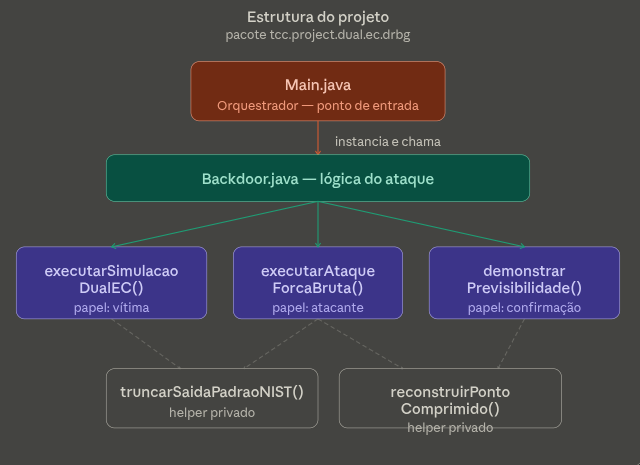
\includegraphics[width=0.8\textwidth]{Modelos/DualEcDRGB/dual_ec_drgb_diagram_code.png}
                    \legend{Fonte: Elaborado pelo autor (2026)}
            \end{figure}
        
            Diagrama é uma representação visual do processo de simulação do backdoor do Dual\_EC\_DRBG. Ele ilustra as etapas envolvidas na geração de números pseudoaleatórios e na execução do ataque de força bruta para recuperar o estado interno.
            Esse processo foi dividido entre a Main como orquestrador e a classe Backdoor, que contém a lógica de simulação e ataque, além de funções auxliares.
            \textbf{Main}: Configura os parâmetros da curva elíptica, pontos P e Q, semente inicial e chama os métodos de simulação e ataque.
            \textbf{Backdoor}: Contém o método executarSimulacaoDualEC para simular a geração de números pseudoaleatórios e o método executarAtaqueForcaBruta para recuperar o estado interno a partir das saídas observadas. 
            Ele também inclui funções auxiliares para reconstruir pontos e truncar saídas conforme o padrão NIST.\@\newline
        
            \begin{figure}[H]
                    \centering
                    \caption{Fluxo da Simulação do Backdoor do Dual\_EC\_DRBG}\label{fig:dual_ec_drgb_process}
                    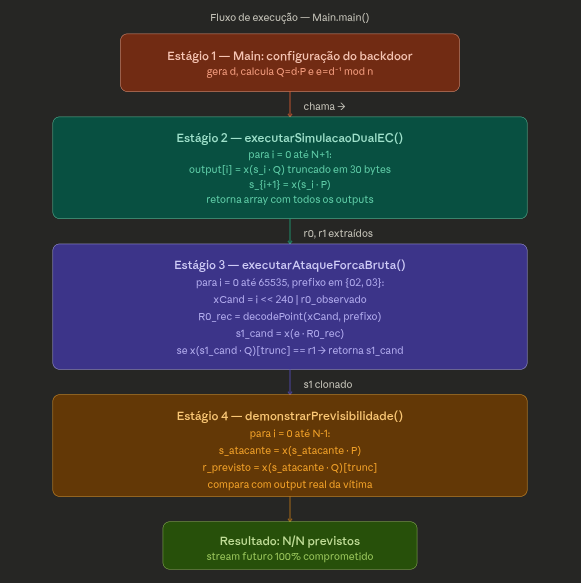
\includegraphics[width=0.8\textwidth]{Modelos/DualEcDRGB/dual_ec_drgb_process.png}
                    \legend{Fonte: Elaborado pelo autor (2026)}
            \end{figure}
        
            Um fluxo de execução é a ordem exata em que as instruções de um programa são processadas pelo computador. Diferente do fluxo original de funcionamento do DUAL\_EC\_DRBG, 
            e como atacantes utilizam sua fragilidade. Na simulação todas as etapas foram implementadas e gerenciadas ao mesmo tempo, se conversando. Na realidade, essas funções e etapas não se conversam. 
            O ataque começa com R0 e R1 (os dois outputs observados). 
            O atacante não olha para R2 durante o processo de quebra — ele prevê R2 de forma independente, 
            e só ao final compara com o valor real para confirmar que acertou. 
            Isso é idêntico ao que aconteceria na vida real: o servidor TLS emite R0 num handshake, R1 num pacote seguinte, e R2 em outro pacote posterior — todos trafegam pela rede, e o atacante os captura em sequência. 
            R2 já chegou pela rede antes mesmo de o atacante terminar o brute-force dos 16 bits.\newline
        
            \begin{figure}[H]
                    \centering
                    \caption{Simulação do Ataque de Força Bruta Teste 1}\label{fig:dual_ec_drbg_backdoor_attack_n1}
                    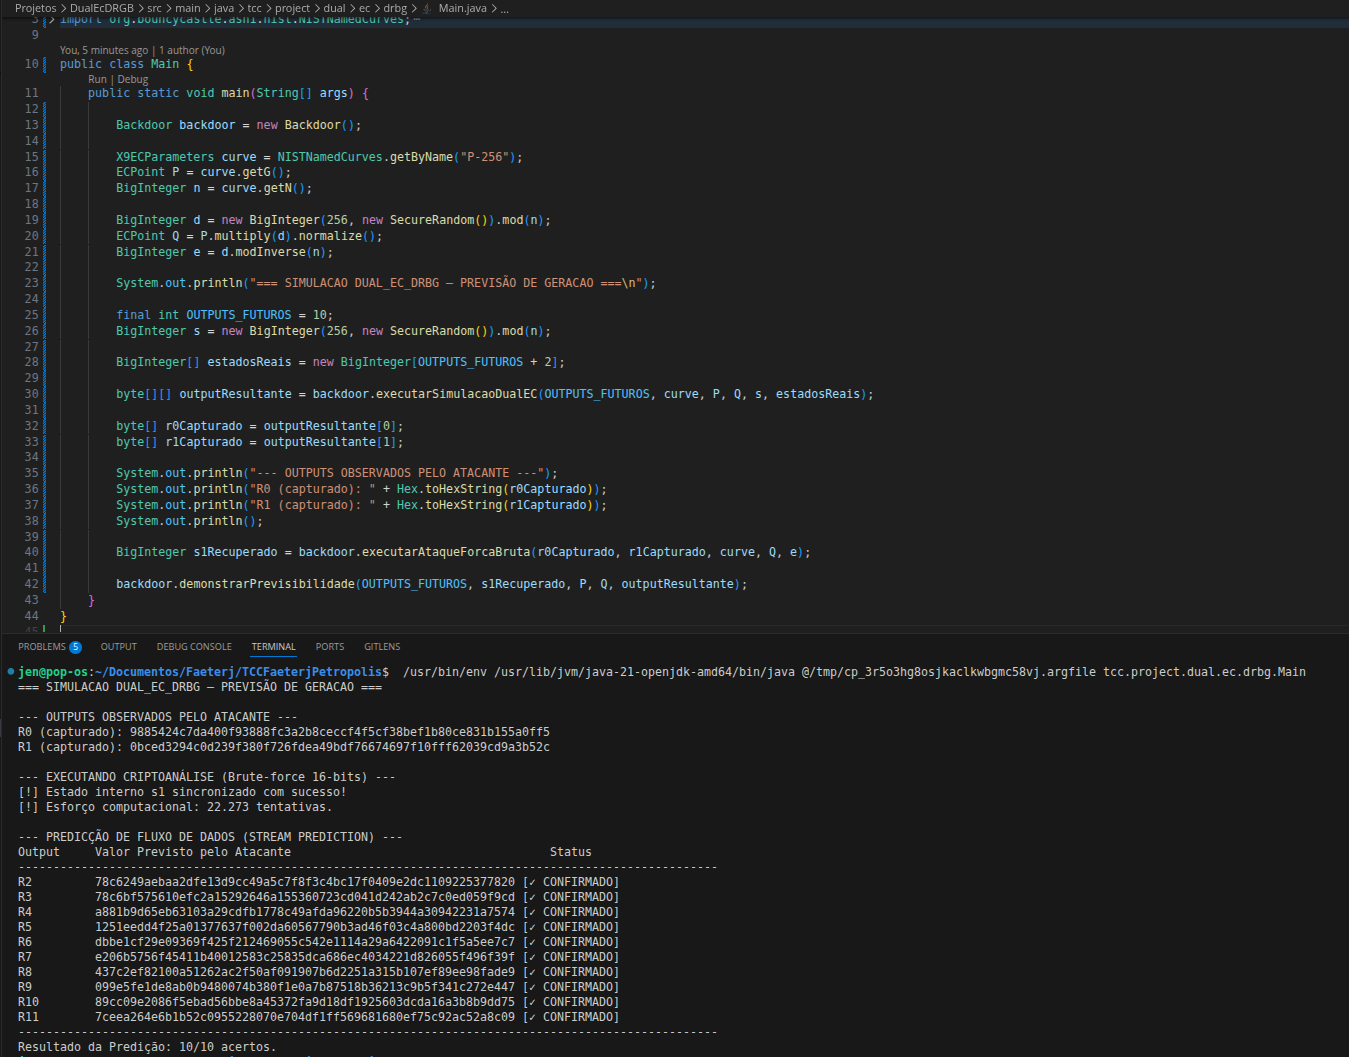
\includegraphics[width=0.7\textwidth]{Modelos/DualEcDRGB/dual_ec_drgb_backdoor_attack_n1.png}
                    \legend{Fonte: Elaborado pelo autor (2026)}
            \end{figure}
        
            A comprovação prática da vulnerabilidade do Dual\_EC\_DRBG durante essa simulação demonstra de forma clara que após o atacante ter acesso aos dois primeiros outputs (R0 e R1), 
            ele pode realizar um ataque de força bruta para recuperar o estado interno do gerador. E com isso ele consegue não só prever o R2, mas também todos os outputs futuros, 
            comprometendo completamente a segurança do sistema que depende desse gerador para suas operações criptográficas.\newline
        
            \begin{figure}[H]
                    \centering
                    \caption{Simulação do Ataque de Força Bruta Teste 2}\label{fig:dual_ec_drbg_backdoor_attack_n2}
                    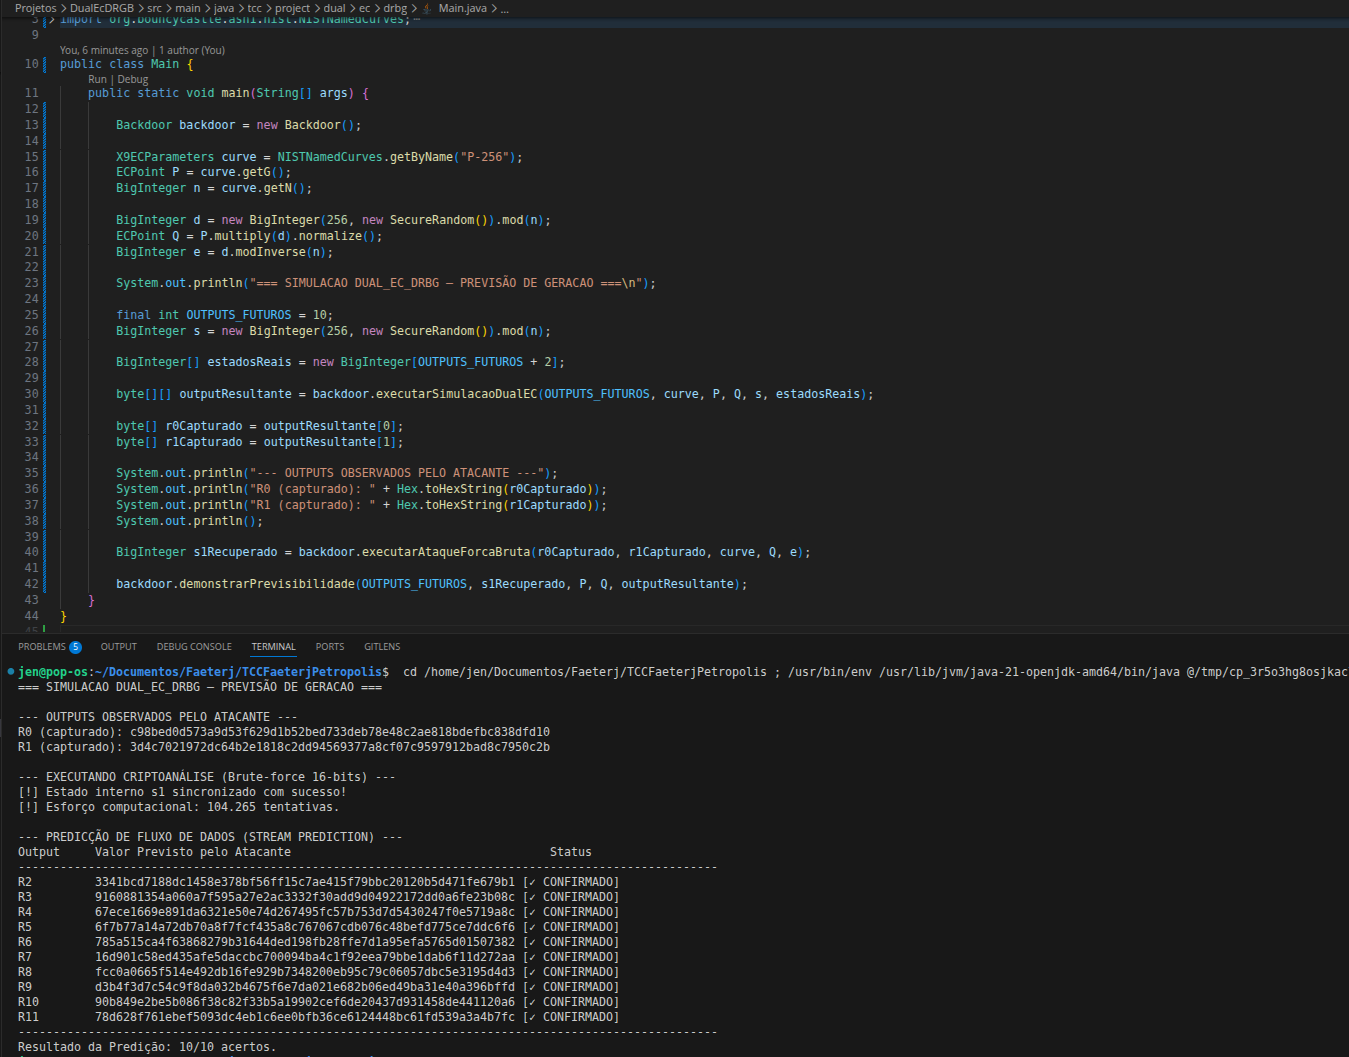
\includegraphics[width=0.8\textwidth]{Modelos/DualEcDRGB/dual_ec_drgb_backdoor_attack_n2.png}
                    \legend{Fonte: Elaborado pelo autor (2026)}
            \end{figure}
        
            Apesar de o truncamento especificado pelo padrão NIST SP 800-90A remover apenas 16 bits da coordenada $x$, o custo efetivo do ataque de recuperação de estado é da ordem de $2^{17}$ multiplicações escalares.   
            Isso ocorre porque, para cada candidato reconstruído de $x$, é necessário considerar ambas as possíveis coordenadas $y$, correspondentes às soluções par e ímpar da equação da curva elíptica.
            Formalmente, o custo total pode ser expresso como:
            \[
            2^{16} \times 2 = 2^{17}
            \]
            No experimento realizado, observou-se que a sincronização do estado exigiu 104.265 tentativas, valor consistente com o limite teórico máximo de 131.072 operações.

        O Bug do Debian OpenSSL (2008): Um desenvolvedor removeu uma linha de código que gerava entropia porque ela causava avisos no depurador. O resultado foi que apenas 32.768 chaves SSH eram possíveis. 
        Um ataque de força bruta levava segundos.
        
        Ataques em Cartões Inteligentes (Taiwan): Milhares de IDs digitais foram gerados com sementes fracas, permitindo que chaves privadas RSA fossem fatoradas a partir das chaves públicas.

        \section{Vulnerabilidades em Algoritmos Criptográficos}

        Algoritmo de grover. capaz de reduzir a forća das entropias das seed pela metade: https://learn.microsoft.com/es-es/azure/quantum/concepts-grovers
        Algoritmo de Grover e a Semente: Explique que o ataque de Grover não "quebra" a matemática do AES ou da Seed, mas reduz a busca exaustiva. 
        Se você usa uma semente de 128 bits, para um computador quântico ela tem o esforço de apenas $2^{64}$. 
        Por isso, o NIST IR 7977 exige o dobro de bits (256).Algoritmo de Shor: Este é o "assassino" do RSA e da Curva Elíptica. 
        Enquanto o Grover reduz a força, o Shor aniquila o RSA completamente. É a razão principal da existência da Criptografia Pós-Quântica (PQC).
        
        Colisões em SHA-1: Cite o projeto SHAttered (Google), que provou na prática que o SHA-1 é inseguro ao gerar dois arquivos PDF diferentes com o mesmo hash.


%\chapter{NIST SP 800-22: Testes de Aleatoriedade para Geradores de Números Pseudoaleatórios}
Bateria de testes SP 800--22 do NIST e o conceito de indistinguibilidade estatística.

        O NIST Test Suite consiste em um pacote de 15 testes de estatistas desenvolvidos para avaliar a as sequencias binarias aleatórias (com comprimento arbitrário),
        gerados por geradores de números aleatórios ou pseudo criptografados, seja de forma em hardware ou software. 
        les podem ser decompostos em vários subtestes de acordo com a necessidade e o tipo de geração aleatória que podem ter uma sequencia. Os 15 testes são:
        \begin{enumerate}
          \item Teste de Frequência (monobit)
          \item Teste de Frequência dentro de um bloco
          \item Teste de Sequencias
          \item Testes para Maior Sequencia de Uns em um bloco
          \item Testes de Posto de Matriz Binária
          \item Teste da Transformada Discreta de Fourier (Espectral)
          \item Teste de Correspondência de Modelos não Sobrepostos
          \item Teste de Correspondência de Modelos Sobrepostos
          \item Teste "Estatístico Universal" de Maurer
          \item Teste de Complexidade Linear
          \item Teste Serial
          \item Teste de Entropia Aproximada
          \item Teste de Somas Cumulativas (Cusums)
          \item Teste de Excursões Aleatórias
          \item Teste de Variante de Excursões Aleatórias
        \end{enumerate}\nocite{NistsTP}

        Falar separadamente sobre cada um dos 15 testes. Mostrando um teste local separado. (Seguir documentacao do guthub para execucao local)\cite{NISTGit}
        
        \subsection{Bateria de Testes}%PASSO 1 - Explicacao de como vai ser efetuado os Testes

            Os arquivos binários gerados em Java servem como a entrada bruta para o NIST SP 800--22, 
            que interpreta os bytes como fluxos contínuos de bits para análise estatística. Ao executar o programa, 
            a ferramenta particiona esses dados em blocos de tamanho fixo, como sequências de $10^{6}$ bits, 
            aplicando sobre cada um deles quinze testes que buscam padrões não aleatórios, como repetições excessivas ou falta de complexidade linear. 
            Para cada teste, o sistema calcula um $P\text{-value}$, que quantifica a probabilidade de a sequência ter sido gerada por um processo puramente aleatório. 
            Ao final, o sucesso do gerador é determinado pela uniformidade desses valores e pela proporção de sequências que mantiveram o $P\text{-value} \geq 0,01$.

            \begin{figure}[htb]
                \centering
                \caption{Modelo simples de um PRNG com LCG}\label{fig:model_prng_lcg}
                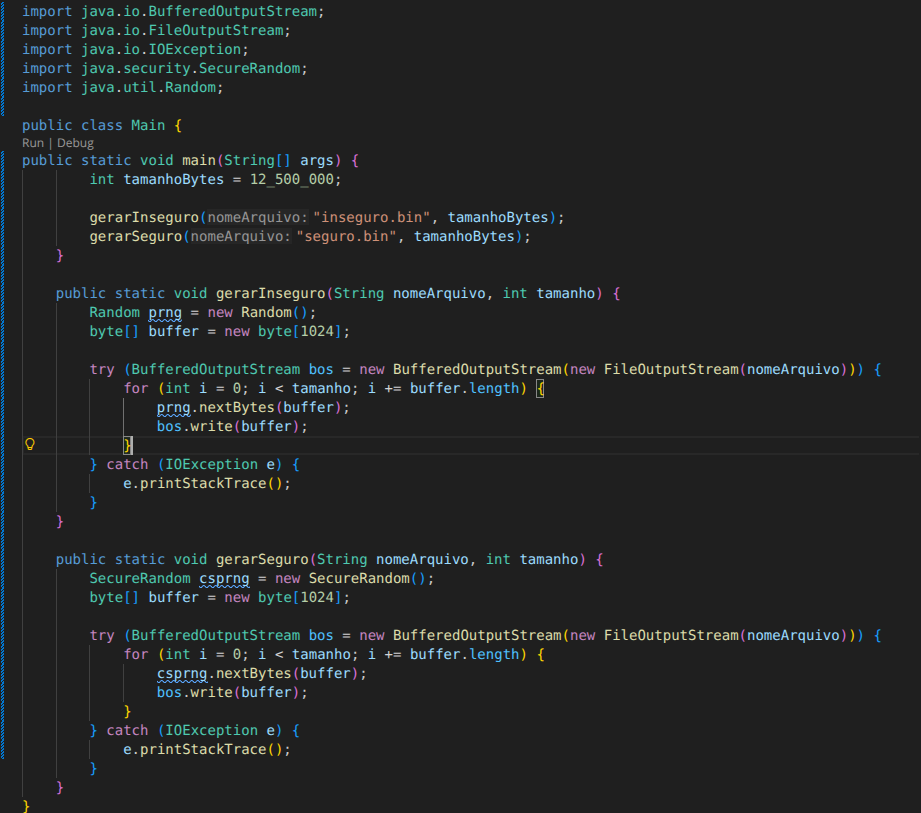
\includegraphics[width=0.8\textwidth]{NIST/gerador_bits_testes_NIST.png}
                \legend{Fonte: Elaborado pelo autor (2026)}
            \end{figure}

        %PASSO 1.1 - Modelo de geracao LCG (voce já fez, tem pronto a explicacao)
        \subsubsection{Random}
        
        A função java.util.Random faz uso do modelo LCG “Gerador Congruencial Linear”. 
        Ele é um modelo puramente matemático. 
        Onde o mesmo é usado para gerar uma sequência de números aleatórios, 
        calculados por uma equação linear.
        \begin{equation}
            x_{i+1} = (A \cdot x_i + C) \pmod{M}
            \label{eq:lca}
        \end{equation}
        Onde o valor inicial “x0” é a seed, 
        A e C são parâmetros inteiros que podem ter um valor 
        já pré-definido ou passados diretamente, 
        M é o espaço dos valores aleatórios possíveis e “mod” é o 
        restante da divisão inteira.
        
        %PASSO 1.3 - Modelo de geracao Seguro usando entropia

        \subsubsection{SegureRandom}
        A função java.security.SegureRandom faz utilização do CSPRNG, que diferente do LCG.\@ Esse tipo de gerador busca caos do hardware.
        Sendo elas interrupçoes de hardware, pressionar das teclas do teclado, posição e movimento do mouse,
        pequenas flutuaçoes de voltagem do processador e/ou o tempo que o disco demora pra fazer a requisição.
        Esses eventos imprevisíveis são misturados, usando funçoes hash como SHA-256 para criar uma seed de alta entropia.
        Mesmo que se conheça o algoritmo, não é possivel recriar o mesmo evento. Justamente pelo fator caos fisico que foi utilizado.

        

\chapter{Revisão dos protocolos e padrões de criptografia}
    \section{Fundamentação da Autoridade e Tipos de Padrões}
        The authority for NIST to develop cryptographic standards and guidelines is derived from the Federal Information Security Management Act (FISMA) of 2002, which requires federal agencies to use standards and guidelines developed by NIST.\@
        NIST develops cryptographic standards and guidelines through a public process that includes soliciting input from stakeholders, conducting research and analysis, and publishing draft documents for public comment. 
        The types of standards and guidelines developed by NIST include Federal Information Processing Standards (FIPS), Special Publications (SP), and Interagency Reports (IR). 
        FIPS are mandatory standards that must be followed by federal agencies, while SPs and IRs are voluntary guidelines that provide recommendations for best practices in cryptography.
        \subsection{FIPS} %capitulo 3 pg 10
            FIPS are developed through a rigorous process that includes public input, testing, and validation. 
            They cover a wide range of topics, including encryption algorithms, key management, and digital signatures. 
            Examples of FIPS include FIPS 140--2, which specifies the security requirements for cryptographic modules, and FIPS 197, which specifies the Advanced Encryption Standard (AES).
        \subsection{SPs} %capitulo 3 pg 10
            SPs are developed to provide guidance on specific topics related to cryptography. 
            They are often developed in response to emerging threats or new technologies, and may cover topics such as secure software development, cryptographic key management, and secure communication protocols. 
            Examples of SPs include SP 800--57, which provides guidelines for key management, and SP 800--175, which provides guidelines for password-based key derivation.
        \subsection{IRs}
            IRs are developed to provide information and analysis on specific topics related to cryptography. 
            They are often developed in response to specific requests from federal agencies or other stakeholders, and may cover topics such as the state of the art in cryptographic research, emerging threats and vulnerabilities, and the impact of new technologies on cryptography. 
            Examples of IRs include IR 7977, which provides an overview of NIST's cryptographic standards and guidelines development process, and IR 8105, which provides an analysis of the security of post-quantum cryptographic algorithms.
        \subsection{ITL} %capitulo 1 pg 06
            The Information Technology Laboratory (ITL) is responsible for developing and maintaining NIST's cryptographic standards and guidelines. 
            ITL conducts research and analysis on cryptographic topics, solicits input from stakeholders, and publishes draft documents for public comment. 
            ITL also provides technical assistance to federal agencies and other stakeholders on the implementation of NIST's cryptographic standards and guidelines.
        \subsection{CSD} %capitulo 1 pg 06
            The Computer Security Division (CSD) is a division within ITL that is responsible for developing and maintaining NIST's cryptographic standards and guidelines. 
            CSD conducts research and analysis on cryptographic topics, solicits input from stakeholders, and publishes draft documents for public comment. 
            CSD also provides technical assistance to federal agencies and other stakeholders on the implementation of NIST's cryptographic standards and guidelines.
    \section{Principios ded Segurança}
        The principles of security that guide NIST's development of cryptographic standards and guidelines include confidentiality, integrity, availability, and non-repudiation. 
        Confidentiality refers to the protection of information from unauthorized access or disclosure. 
        Integrity refers to the protection of information from unauthorized modification or destruction. 
        Availability refers to the protection of information from unauthorized disruption or denial of service. 
        Non-repudiation refers to the ability to prove that a specific action or event occurred, and that it was performed by a specific individual or entity.
        \subsection{Mérito Técnico e Provas de Segurança} %capitulo 2 pg 7-8
            NIST evaluates the technical merit and security of cryptographic algorithms and protocols through a rigorous process that includes public input, testing, and validation. 
            NIST conducts research and analysis on cryptographic topics, solicits input from stakeholders, and publishes draft documents for public comment. 
            NIST also conducts testing and validation of cryptographic algorithms and protocols to ensure that they meet the required security standards.
        \subsection{Integridade e Influência} %capitulo 2 pg 7
            NIST's cryptographic standards and guidelines are designed to ensure the integrity of information and to influence the development of secure technologies. 
            NIST's standards and guidelines provide a framework for the development of secure technologies, and they help to ensure that information is protected from unauthorized access, modification, or destruction. 
            NIST's standards and guidelines also help to promote the adoption of secure technologies by providing a common framework for developers and users.
    \section{Metodologia de Seleção}
        NIST's methodology for selecting cryptographic algorithms and protocols is based on a rigorous process that includes public input, testing, and validation. 
        NIST solicits input from stakeholders, including industry experts, academia, and government agencies, to identify potential candidates for cryptographic algorithms and protocols. 
        NIST then conducts research and analysis on the candidates to evaluate their technical merit and security. 
        NIST also conducts testing and validation of the candidates to ensure that they meet the required security standards. 
        Finally, NIST publishes draft documents for public comment to solicit feedback from stakeholders before finalizing the selection of cryptographic algorithms and protocols.
        \subsection{Competições de Algoritmos} %capitulo 5 pg 13/ capitulo 7 pg 18
            NIST has conducted several competitions to select cryptographic algorithms and protocols, including the Advanced Encryption Standard (AES) competition and the Post-Quantum Cryptography (PQC) competition. 
            The AES competition was held in the late 1990s to select a new encryption algorithm to replace the aging Data Encryption Standard (DES). 
            The PQC competition is currently underway to select new cryptographic algorithms that are resistant to attacks by quantum computers.
        \subsection{Fases de Competição} % capitulo 7 pg 24
            The phases of NIST's competitions for cryptographic algorithms and protocols typically include a call for submissions, an initial evaluation phase, a public comment period, and a final selection phase. 
            During the call for submissions, NIST solicits input from stakeholders to identify potential candidates for cryptographic algorithms and protocols. 
            During the initial evaluation phase, NIST conducts research and analysis on the candidates to evaluate their technical merit and security. 
            During the public comment period, NIST publishes draft documents for public comment to solicit feedback from stakeholders. 
            Finally, during the final selection phase, NIST evaluates the feedback received during the public comment period and makes a final selection of cryptographic algorithms and protocols.
        \subsection{Propriedade Intelectual (IP)} %capitulo 7 pg 23
            NIST's approach to intellectual property (IP) in the context of cryptographic standards and guidelines is to encourage the use of open standards and to avoid the use of proprietary algorithms and protocols. 
            NIST's standards and guidelines are designed to be freely available and to promote interoperability among different technologies. 
            NIST also encourages the use of open-source software and hardware implementations of cryptographic algorithms and protocols to promote transparency and security.
    \section{Manutenção e Substituição de Padrões}
        NIST's process for maintaining and replacing cryptographic standards and guidelines is based on a continuous review and evaluation process. 
        NIST regularly reviews its standards and guidelines to ensure that they remain relevant and effective in the face of emerging threats and new technologies. 
        When necessary, NIST may update or replace its standards and guidelines to address new threats or to take advantage of new technologies. 
        NIST also provides technical assistance to federal agencies and other stakeholders on the implementation of its standards and guidelines to ensure that they are effectively implemented and maintained over time.
        \subsection{Ciclo de Vida e Retirada (Withdrawal)} %capitulo 7 pg 26
            The lifecycle of NIST's cryptographic standards and guidelines typically includes several stages, including development, publication, implementation, maintenance, and withdrawal. 
            During the development stage, NIST solicits input from stakeholders and conducts research and analysis to develop new standards and guidelines. 
            During the publication stage, NIST publishes draft documents for public comment and finalizes the standards and guidelines based on feedback received. 
            During the implementation stage, federal agencies and other stakeholders implement the standards and guidelines in their systems and technologies. 
            During the maintenance stage, NIST regularly reviews its standards and guidelines to ensure that they remain relevant and effective. 
            Finally, during the withdrawal stage, NIST may retire or replace standards and guidelines that are no longer effective or relevant.
        \subsection{Análise de Constantes e Proveniência} %capitulo 7 pg 22
            NIST's process for analyzing the constants and provenance of cryptographic algorithms and protocols is based on a rigorous evaluation process that includes public input, testing, and validation. 
            NIST evaluates the constants used in cryptographic algorithms and protocols to ensure that they are secure and do not introduce vulnerabilities. 
            NIST also evaluates the provenance of cryptographic algorithms and protocols to ensure that they are developed by reputable sources and do not have hidden weaknesses or backdoors.
    

\chapter{Planejamento para a Criptografia Pós-Quântica (PQC)}

\section{Contextualização e Gestão de Risco}
Esta seção introduz o problema e explica por que a transição deve ser planejada imediatamente, abordando o cenário de risco sob a ótica organizacional.

\subsection{A Ameaça Quântica e o Paradigma ``Harvest Now, Decrypt Later''}
\textbf{Conteúdo:} Explicação sobre como adversários já estão coletando tráfego cifrado atual para quebrar a criptografia assim que computadores quânticos criptograficamente relevantes (CRQC) estiverem disponíveis.\\
\textbf{Documento indicado:} \textit{NIST SP 1800-38A (Executive Summary)}. Fornece o panorama do problema e a urgência da migração sob a perspectiva do NCCoE.

\subsection{Mapeamento do Risco Quântico}
\textbf{Conteúdo:} Como integrar a ameaça quântica nos processos de gestão de risco cibernético da organização.\\
\textbf{Documento indicado:} \textit{NIST CSWP 48 (Cybersecurity White Paper)}. Relaciona a migração PQC com as práticas do \textit{NIST Cybersecurity Framework (CSF)}.

\section{Inventário e Descoberta Criptográfica}
Antes de migrar, uma organização precisa saber o que possui. Esta seção detalha as metodologias para rastrear o uso atual de criptografia.

\subsection{Estratégias de Descoberta em Redes e Sistemas}
\textbf{Conteúdo:} Métodos e ferramentas para varrer infraestruturas, encontrar chaves embutidas em código, protocolos obsoletos e certificados ocultos.\\
\textbf{Documento indicado:} \textit{NIST SP 1800-38B (Discovery for PQC Migration)}. Fornece cenários práticos e arquiteturas de referência para a fase de descoberta.

\subsection{Adoção do CBOM (Cryptographic Bill of Materials)}
\textbf{Conteúdo:} O conceito de catalogar a criptografia de forma padronizada para monitorar vulnerabilidades em cadeias de suprimentos de software.\\
\textbf{Documento indicado:} \textit{NIST SP 1800-38B}. Aborda diretamente como gerar e manter inventários de ativos criptográficos.

\section{Agilidade Criptográfica e Novos Padrões}
Aborda o planejamento arquitetural necessário para facilitar atualizações e apresenta as novas ferramentas de proteção.

\subsection{Conceitos de Agilidade e Desafios de Desempenho}
\textbf{Conteúdo:} O que significa projetar um sistema ágil e quais são os impactos reais na rede (latência, tamanho de chaves, largura de banda) ao trocar os algoritmos.\\
\textbf{Documento indicado:} \textit{NIST SP 1800-38C (Interoperability and Performance)}. Apresenta casos de uso reais e testes de impacto.

\subsection{Os Padrões Pós-Quânticos Finais}
\textbf{Conteúdo:} A especificação técnica e a indicação de uso dos algoritmos selecionados.\\
\textbf{Documentos indicados:}
\begin{itemize}
    \item \textbf{FIPS 203 (ML-KEM):} Para troca de chaves criptográficas.
    \item \textbf{FIPS 204 (ML-DSA) e FIPS 205 (SLH-DSA):} Para assinaturas digitais.
    \item \textbf{NIST IR 8413:} Para critérios técnicos do Round 3.
\end{itemize}

\section{Estratégias de Migração e Hibridização}
Foca na parte prática e operacional da transição.

\subsection{Hibridização (Criptografia Clássica e PQC)}
\textbf{Conteúdo:} A abordagem recomendada de usar algoritmos clássicos em conjunto com PQC durante o período de transição.\\
\textbf{Documento indicado:} \textit{NIST SP 1800-38C}. Discute os protocolos que suportam negociação híbrida.

\subsection{Assinaturas Baseadas em Hash para Adoção Imediata}
\textbf{Conteúdo:} Uso de algoritmos de assinatura que já são considerados seguros contra ataques quânticos, úteis para validar firmware.\\
\textbf{Documento indicado:} \textit{NIST SP 800-208}. Padrões stateful hash-based (LMS e XMSS).

\section{Roadmap e Manutenção da Base Criptográfica}
Conclui o planejamento com prazos normativos e a importância de elementos basilares da criptografia.

\subsection{Cronograma e Descontinuação de Algoritmos Atuais}
\textbf{Conteúdo:} Prazos para que algoritmos de chaves públicas atuais (como RSA-2048) deixem de ser considerados seguros.\\
\textbf{Documento indicado:} \textit{NIST SP 800-131A Rev. 3}. Estipula o ciclo de vida e os prazos limite.

\subsection{O Papel Contínuo da Entropia}
\textbf{Conteúdo:} A garantia de que a segurança fundamental ainda depende da geração de números aleatórios de alta qualidade (RNG).\\
\textbf{Documento indicado:} \textit{NIST SP 800-22}. Conecta os testes de aleatoriedade como pré-requisito indispensável.

\chapter{NIST IR 8547  Transição para a Criptografia Pós-Quântica: Estratégias e Considerações}
    \section{Urgencia Prática e o Modelo de Ameaça}
        O modelo de ameaça é uma ferramenta essencial para a segurança cibernética, permitindo que as organizações identifiquem, compreendam e mitiguem ameaças potenciais.
        Ele ajuda a priorizar os recursos de segurança, focando nas ameaças mais relevantes e perigosas.
        O modelo de ameaça é fundamental para o desenvolvimento de estratégias eficazes de defesa cibernética, garantindo que as organizações estejam preparadas para enfrentar os desafios atuais e futuros.
        \subsection{Ameaça Harvest now, Decrypt Later} %capitulo 1 pg 8
            A ameaça "Harvest now, Decrypt Later" refere-se à prática de coletar dados criptografados agora, com a intenção de descriptografá-los no futuro, quando os recursos computacionais ou as vulnerabilidades de segurança permitirem.
            Essa ameaça é particularmente preocupante para dados sensíveis que precisam ser protegidos por longos períodos, como informações pessoais, financeiras e de saúde.
            Para mitigar essa ameaça, é crucial adotar práticas de criptografia robustas e atualizadas, além de monitorar continuamente as vulnerabilidades e avanços tecnológicos que possam impactar a segurança dos dados.
        \subsection{Teorema de Mosca e a Linha do Tempo} %capitulo 3 pg 14
            O Teorema de Mosca é um conceito fundamental na segurança cibernética que destaca a importância de considerar o tempo ao avaliar ameaças e vulnerabilidades.
            Ele sugere que, para proteger adequadamente os sistemas, é necessário entender não apenas as ameaças atuais, mas também as ameaças futuras que podem surgir à medida que a tecnologia evolui.
            A linha do tempo é uma ferramenta útil para visualizar e planejar a defesa contra ameaças, permitindo que as organizações antecipem e se preparem para possíveis ataques futuros, garantindo uma postura de segurança proativa.
    \section{Novos Padrões e Categorias de Segurança}
        A evolução dos padrões de segurança é crucial para enfrentar as ameaças cibernéticas em constante mudança.
        Novos padrões e categorias de segurança são desenvolvidos para abordar as vulnerabilidades emergentes e garantir a proteção eficaz dos sistemas e dados.
        A adoção de padrões atualizados é essencial para manter a resiliência contra ataques cibernéticos, promovendo uma abordagem de segurança mais robusta e adaptável às novas ameaças.
        \subsection{Publicações dos primeiros FIPS PQC} %capitulo 1 pg 8
            As publicações dos primeiros FIPS (Federal Information Processing Standards) para criptografia pós-quântica (PQC) representam um marco importante na evolução da segurança cibernética.
            Esses padrões são desenvolvidos para garantir que os sistemas de criptografia sejam resistentes a ataques de computadores quânticos, que têm o potencial de quebrar os métodos de criptografia tradicionais.
            A adoção desses padrões é crucial para proteger dados sensíveis e garantir a segurança a longo prazo, especialmente à medida que a tecnologia quântica avança e se torna mais acessível.
        \subsection{Categorias de Segurança Pós-Quântica (1 a 5)} %capitulo 4.1 pg 19
            As categorias de segurança pós-quântica são classificações que ajudam a identificar e categorizar os diferentes tipos de algoritmos de criptografia que são resistentes a ataques de computadores quânticos.
            Essas categorias incluem algoritmos baseados em reticulados, códigos, multivariados, hash-based e isogenias, cada um com suas próprias características e níveis de segurança.
            A compreensão dessas categorias é essencial para escolher os algoritmos mais adequados para proteger dados sensíveis contra ameaças futuras, garantindo uma postura de segurança robusta e resiliente.
    \section{Cronograma de Descontinuação (Deprecation)}
        O cronograma de descontinuação é um plano estratégico que define o processo e os prazos para a retirada de sistemas, tecnologias ou práticas de segurança obsoletas.
        Ele é essencial para garantir uma transição suave e segura para novas soluções, minimizando os riscos associados à manutenção de sistemas vulneráveis ou desatualizados.
        A implementação de um cronograma de descontinuação eficaz ajuda as organizações a se adaptarem às mudanças tecnológicas e a manterem uma postura de segurança proativa, garantindo a proteção contínua dos dados e sistemas.
        \subsection{Transição de Assinaturas Digitais (RSA, ECDSA, EdDSA)} %Capítulo 4.1.1, Página 20, Tabela 2.
            A transição de assinaturas digitais, como RSA, ECDSA e EdDSA, é um processo crucial para garantir a segurança dos sistemas de criptografia à medida que novas ameaças emergem.
            Com o avanço da tecnologia, especialmente a computação quântica, é necessário migrar para algoritmos de assinatura digital mais robustos e resistentes a ataques futuros.
            A adoção de novos algoritmos de assinatura digital é essencial para proteger a integridade e autenticidade dos dados, garantindo a segurança a longo prazo em um ambiente cibernético em constante evolução.
        \subsection{Transição de Estabelecimento de Chaves (DH, MQV, RSA)} %Capítulo 4.1.2, Página 21, Tabela 4.
            A transição de estabelecimento de chaves, como DH (Diffie-Hellman), MQV (Menezes-Qu-Vanstone) e RSA, é um processo fundamental para garantir a segurança das comunicações criptografadas.
            Com o avanço da tecnologia, especialmente a computação quântica, é necessário migrar para algoritmos de estabelecimento de chaves mais robustos e resistentes a ataques futuros.
            A adoção de novos algoritmos de estabelecimento de chaves é essencial para proteger a confidencialidade e integridade das comunicações, garantindo a segurança a longo prazo em um ambiente cibernético em constante evolução.
    \section{Estratégias de Transição: Protocolos Hibridos}
        As estratégias de transição, como os protocolos híbridos, são abordagens que combinam algoritmos de criptografia tradicionais com algoritmos pós-quânticos para garantir a segurança durante o processo de migração.
        Esses protocolos permitem que as organizações mantenham a compatibilidade com sistemas legados enquanto adotam novas soluções de segurança, minimizando os riscos associados à transição.
        A implementação de protocolos híbridos é uma estratégia eficaz para garantir a proteção contínua dos dados e sistemas durante a evolução da tecnologia, proporcionando uma transição suave e segura para o futuro da segurança cibernética.
        \subsection{Soluções Hibridas (PQC-Classical)} %Capítulo 3.2, Páginas 15-17.
            As soluções híbridas, que combinam algoritmos de criptografia pós-quântica (PQC) com algoritmos clássicos, são uma abordagem estratégica para garantir a segurança durante a transição para novas tecnologias de criptografia.
            Essas soluções permitem que as organizações mantenham a compatibilidade com sistemas legados enquanto adotam novas soluções de segurança, minimizando os riscos associados à migração.
            A implementação de soluções híbridas é essencial para proteger os dados e sistemas durante a evolução da tecnologia, garantindo uma transição suave e segura para o futuro da segurança cibernética.
        \subsection{Protocolos Hibridos (TLS, SSH, IPsec)} %Procura em outro lugar
            Os protocolos híbridos, como TLS (Transport Layer Security), SSH (Secure Shell) e IPsec (Internet Protocol Security), são abordagens que combinam algoritmos de criptografia tradicionais com algoritmos pós-quânticos para garantir a segurança durante a transição para novas tecnologias de criptografia.
            Esses protocolos permitem que as organizações mantenham a compatibilidade com sistemas legados enquanto adotam novas soluções de segurança, minimizando os riscos associados à migração.
            A implementação de protocolos híbridos é essencial para proteger os dados e sistemas durante a evolução da tecnologia, garantindo uma transição suave e segura para o futuro da segurança cibernética.
        \subsection{Agilidade Criptográfica em Camadas de Infraestrutura} %Capítulo 2.2, Páginas 12-13.
            A agilidade criptográfica em camadas de infraestrutura é uma abordagem que permite a flexibilidade na escolha e implementação de algoritmos de criptografia em diferentes camadas de um sistema.
            Essa abordagem é crucial para garantir a segurança durante a transição para novas tecnologias de criptografia, permitindo que as organizações adotem soluções híbridas e se adaptem às mudanças nas ameaças cibernéticas.
            A implementação da agilidade criptográfica em camadas de infraestrutura é essencial para proteger os dados e sistemas durante a evolução da tecnologia, garantindo uma transição suave e segura para o futuro da segurança cibernética.


\chapter{Cristals Kyber}
\section{Introdução}

%Da pra fazer um teste praticoooo: https://github.com/pq-crystals/kyber
% A nist usa, mas nào achei docs deles, vai ter que fazer só o teste pratico e coemntar quea  nist está adotando pra PQC, SE VIRAAAA!!! Comentario dee IA: e que o kyber é um dos candidatos a ser o padrao de criptografia pós-quântica do nist, e que é baseado em problemas de aprendizado com erros (LWE) e é considerado resistente a ataques de computadores quânticos.


O CRYSTALS-Kyber é um sistema de criptografia de chave pública baseado em problemas de aprendizado com erros (LWE) e é considerado resistente a ataques de computadores quânticos. 
Ele é parte do projeto CRYSTALS (Cryptographic Suite for Algebraic Lattices) e é um dos candidatos para o padrão de criptografia pós-quântica do NIST (National Institute of Standards and Technology). O CRYSTALS-Kyber é projetado para ser eficiente em termos de tempo de execução e tamanho de chave, tornando-o uma opção viável para aplicações práticas de criptografia pós-quântica.
\section{Estrutura do CRYSTALS-Kyber}
O CRYSTALS-Kyber é baseado em um esquema de criptografia de chave pública que utiliza matrizes e vetores para realizar operações de criptografia e descriptografia. Ele é composto por três algoritmos principais: geração de chaves, criptografia e descriptografia.

\chapter{CRIPTOGRAFIA PÓS-QUÂNTICA (PQC)} % Capitulo 5

    \section{Definição e Objetivos da PQC}

    Algoritmos clássicos projetados para resistir a ataques quânticos.

    \section{Paradigmas Matemáticos da PQC}

    Reticulados, códigos corretores de erro, funções hash e isogenias.

    \section{Criptografia Baseada em Reticulados}

    Introdução ao conceito de Lattices como base da nova segurança criptográfica.

    \section{Learning With Errors (LWE)}

    Fundamento matemático da pseudoaleatoriedade pós-quântica.

    \subsection{Implementação Didática em Java (Demonstração)}

    Implementação simplificada do LWE do zero em Java para fins didáticos, mostrando como o erro intencional funciona matematicamente antes de utilizar a biblioteca pronta.

    \section{Padronização Pós-Quântica}

    O papel do ML-KEM (Kyber) e o processo de padronização conduzido pelo NIST.

\chapter{A TRANSIÇÃO PARA PQC NO ECOSSISTEMA JAVA} % Capitulo 6

    \section{Suporte à Criptografia Pós-Quântica no Java}

    Evolução do JDK e integração de algoritmos pós-quânticos em versões modernas (Java 21+).

    \section{Crypto-Agility}

    Boas práticas para desenvolvimento de sistemas criptográficos flexíveis e preparados para mudanças de algoritmo.

    \subsection{Implementação Prática: Demo de Crypto-Agility}

    Criação de uma interface Java que abstrai o algoritmo de geração de chaves, permitindo trocar de RSA para Kyber alterando apenas a configuração — sem reescrever o código da aplicação.

    \section{Comparativo de Modelos}

    Geração de chaves e aleatoriedade no modelo clássico versus modelo baseado em reticulados (Module-Lattice).

    \subsection{Implementação Prática: Benchmark Clássico vs. Kyber}

    Benchmark comparativo entre java.security.SecureRandom clássico e ML-KEM (Kyber) via Bouncy Castle, medindo tempo de geração de chaves, uso de memória e throughput. 
    Inclui comparativo de tamanho de chaves entre RSA-2048 e Kyber.
    Nota: Confirmar com o orientador o uso da biblioteca Bouncy Castle como dependência, por ser a opção mais acessível para PQC em Java atualmente.

\chapter{DISCUSSÃO E ANÁLISE CRÍTICA} % Capitulo 7

    \section{Impacto em Desempenho}

    Custos computacionais, consumo de memória e latência — baseados nos resultados do benchmark da seção 6.3.1.

    \section{Barreiras de Adoção}

    Sistemas legados, limitações de hardware e resistência organizacional.

    \section{Implicações Sociais e Éticas}

    Soberania de dados, privacidade, vigilância e assimetria tecnológica.

\chapter{CONCLUSÃO} % Capitulo 8 - Conclusao

    \section{Síntese dos Resultados}

    A inevitabilidade da transição criptográfica.

    \section{Resposta ao Problema de Pesquisa}

    A evolução da pseudoaleatoriedade como pilar da segurança pós-quântica.

    \section{Trabalhos Futuros}

    Geradores Quânticos de Números Aleatórios (QRNG) e integração híbrida TRNG + PQC.

% --- ELEMENTOS PÓS-TEXTUAIS ---
\postextual
%\nocite{*}
\bibliography{referencias}% Arquivo .bib com suas fontes

\end{document}